\documentclass[12pt,a4paper]{article}
\usepackage[english, science, large]{../template/ku-frontpage}
\usepackage{tabularx}
\usepackage{ltablex}
\usepackage{enumitem}
\usepackage[cache=false]{minted}
\setminted[erlang]{
frame=lines,
framesep=2mm,
baselinestretch=1.1,
fontsize=\footnotesize,
linenos,
breaklines}
\usemintedstyle{friendly}
\hypersetup{
    colorlinks=false,
    pdfborder={0 0 0},
}
\begin{document}

\title{ACS Programming Assignment 1}
\subtitle{}

\author{Kai Arne S. Myklebust, Silvan Adrian}
\date{Handed in: \today}
	
\maketitle
\tableofcontents

\section{Questions for Discussion on Architecture}

\subsection{Question 1}

\subsubsection{(a)}
\textbf{Implementation}
\begin{itemize}
	\item \textbf{rateBooks:} We use an additional validate method. Which takes a book rating and validates it by checking if the rating is between (0 - 5) and use the ISBN validation method. If there is a validation error we throw an exception (BookStoreException), this way we either save all or none of the ratings.
	\item \textbf{getTopRatedBooks:} We only check if the number of Books is a positive number ($\geq$ 0).
	\item \textbf{getBooksInDemand:} No Parameter validation. We used streams filtered by missed sales and return an immutable book.
\end{itemize}
\textbf{Tests}
\begin{itemize}
	\item \textbf{rateBooks:} We created the test case \textbf{shouldRateNoBook}, which rates the same book 2 times but one of the ratings is not valid. So no books are rated (total rating: 0, number of times rated: 0)
	\item \textbf{getTopRatedBooks:} We have the test case \textbf{shouldReturnAllTopRatedBooks} which just returns all top rated books (according to the parameter number of books).
	\item \textbf{getBooksInDemand:} We have a test case \textbf{shouldGetBooksInDemand} which just gets all the books in demand.
\end{itemize}

\subsubsection{(b)}
We did that by asserting the results which we get back from the service, so in case we set the local flag true or false. The tests will run either way (stay green).

\subsection{Question 2}
\subsubsection{(a)}
By using a Client/Server architecture, we achieve modularity even though technically the server saves all the books only in the memory. This doesn't allow for multiple servers using the same data (having not a single Database).
\subsubsection{(b)}
It distinguishes between mutable and immutable books, so that the bookstore clients are not allowed to mutate data only get immutable books (no writing is allowed).
\subsubsection{(c)}
If an error occurs in either a client or the service it would mean that both of them will shutdown/fail since they run on the same JVM.
\subsection{Question 3}
\subsubsection{(a)}
The message Handler provides a naming service, so that we are able to use message tags which then executes the corresponding method.
\subsubsection{(b)}
The client calls the server by its server address + a message tag. So the message tag sent by the client decides on which operation gets run on the server.
\subsection{Question 4}
In the Architecture "at-most-once" RPC semantics is implemented, this we see since there are operations which have side-effects (operations which change the state on the server).
In case of failure the operation won't be completed.
\subsection{Question 5}
\subsubsection{(a)}
Yes it is safe to use web proxies with the architecture.
\subsubsection{(b)}
Since the communication between the clients and the Server is already HTTP based it is safe to place web proxies in between the clients and the server.
To the communication itself it doesn't matter if it get gets passed through a proxy before it arrives at the server.

Possible placement of proxies:
\begin{figure}[htb!]
	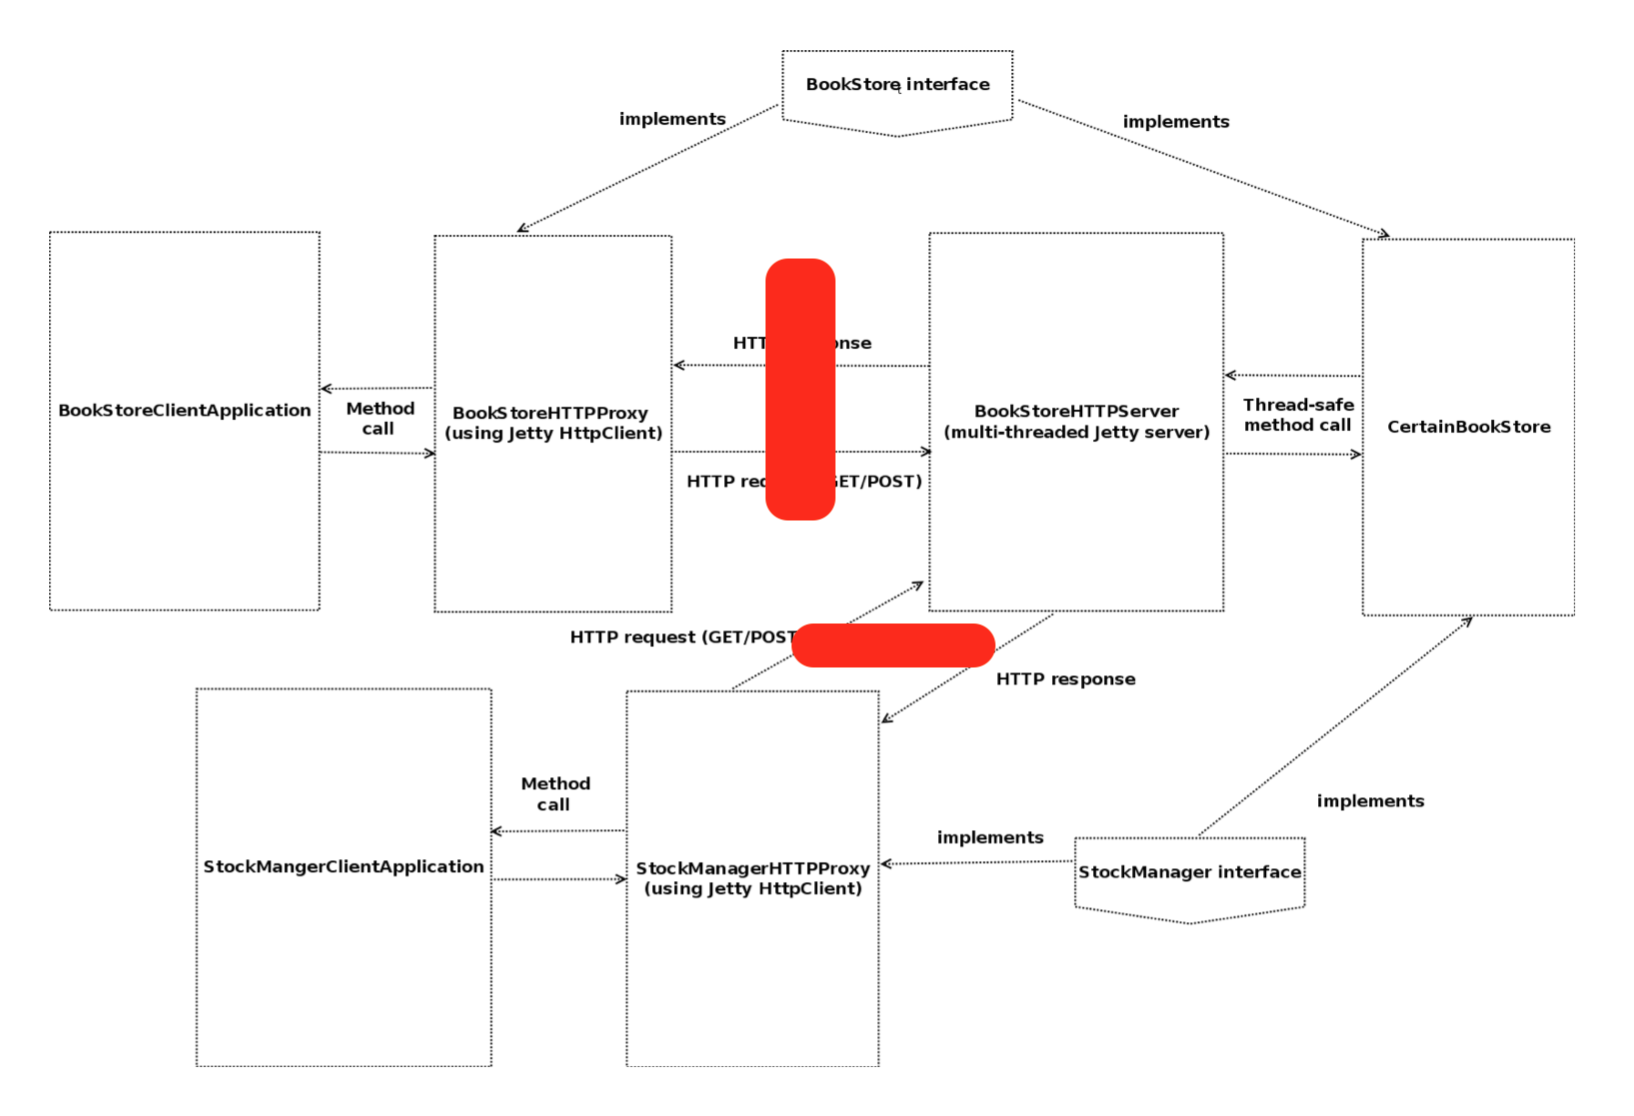
\includegraphics[width=\textwidth]{proxies}
	\caption{Placement of proxies in architecture}
\end{figure}

\subsection{Question 6}
\subsubsection{(a)}
Yes there is a bottleneck in the architecture.
\subsubsection{(b)}
The bottleneck is the server, since its state is hold in the memory, so it can't be scaled. If there are too many clients the server could run out of memory.
Same for the amount of request the server can process, since it can't be scaled horizontally only vertically.
\subsection{Question 7}
\subsubsection{(a)}
Yes failures would be experienced differently since the proxy can handle failures of communicating with the server itself.
The client could then get a failure response from the proxy.
\subsubsection{(b)}
Yes it could, by responding to requests from clients by using it's cache (so the server doesn't even need to be contacted).
\subsubsection{(c)}
Using a web cache won't affect the semantics, since the semantics depends on the state on the server.
For example when buying a book, the state on the server still needs to be updated.
\end{document}}